%% LaTeX2e class for student theses
%% sections/evaluation.tex
%% 
%% Karlsruhe Institute of Technology
%% Institute for Program Structures and Data Organization
%% Chair for Software Design and Quality (SDQ)
%%
%% Dr.-Ing. Erik Burger
%% burger@kit.edu
%%
%% Version 1.3.5, 2020-06-26

\chapter{Regression}
\label{ch:Regression}

After extracting features from the elements, the next step is do learn from the data.
The goal of this Bachelor's thesis is to predict the activation barrier of a catalyst molecule.
The techniques used however are not limited to the activation barrier, 
as it can be expected that other properties of the molecule could be predicted with similar techniques.

For regression, artificial neural networks(ANNs) will be used.
Neural networks have seen a huge surge in popularity in recent years for their ability to 
adapt to high dimensional input data.
The concept is derived from biological neural networks such as the ones found in the human brain.

ANNs are a composed of a set of interconnected neurons.
Each neuron has a set of inputs $x_1 .. x_n$, a bias $b$, and an activation function $f(x)$.
The output will be the result of the activation function applied to the sum of all inputs plus the bias.

$$ y = f \left( \sum_i x_i + b \right) $$

Neurons are grouped together in layers, where the output of each layer is connected to the input of the next one.
For a single prediction, the example is applied to the input layer, the network is then flooded until the output layer is reached.
In the case of regression used here, the value of the output layer is the prediction of the neural network.

% Listing 2: Tex for neural network pipeline
\begin{tikzpicture}[
    % define styles    
    init/.style={ 
         draw, 
         circle, 
         inner sep=2pt,
         font=\Huge,
         join = by -latex
    },
    squa/.style={ 
        font=\Large,
        join = by -latex
    }
]
% Top chain x1 to w1
\begin{scope}[start chain=1]
    \node[on chain=1] at (0,1.5cm)  (x1) {$x_1$};
    \node[on chain=1,join=by o-latex] (w1) {$w_1$};
\end{scope}
% Middle chain x2 to output
\begin{scope}[start chain=2]
    \node[on chain=2] (x2) {$x_2$};
    \node[on chain=2,join=by o-latex] {$w_2$};
    \node[on chain=2,init] (sigma) {$\displaystyle\Sigma$};
    \node[on chain=2,squa,label=above:{\parbox{2cm}{\centering Activation\\ function}}]   {$f_{act}$};
    \node[on chain=2,squa,label=above:Output,join=by -latex] {$y_{out}$};
\end{scope}
% Bottom chain x3 to w3
\begin{scope}[start chain=3]
    \node[on chain=3] at (0,-1.5cm) 
    (x3) {$x_3$};
    \node[on chain=3,label=below:Weights,join=by o-latex]
    (w3) {$w_3$};
\end{scope}
% Bias
\node[label=above:\parbox{2cm}{\centering Bias \\ $b$}] at (sigma|-w1) (b) {};
% Arrows joining w1, w3 and b to sigma
\draw[-latex] (w1) -- (sigma);
\draw[-latex] (w3) -- (sigma);
\draw[o-latex] (b) -- (sigma);
% left hand side brace
\draw[decorate,decoration={brace,mirror}] (x1.north west) -- node[left=10pt] {Inputs} (x3.south west);

\end{tikzpicture}



% Listing 1: Tex for neural network layers
\begin{tikzpicture}[
    % define styles 
    clear/.style={ 
        draw=none,
        fill=none
    },
    net/.style={
        matrix of nodes,
        nodes={ draw, circle, inner sep=10pt },
        nodes in empty cells,
        column sep=2cm,
        row sep=-9pt
    },
    >=latex
]
% define matrix mat to hold nodes
% using net as default style for cells
\matrix[net] (mat)
{
% Define layer headings
|[clear]| \parbox{1.3cm}{\centering Input\\layer} 
   & |[clear]| \parbox{1.3cm}{\centering Hidden\\layer} 
   & |[clear]| \parbox{1.3cm}{\centering Output\\layer} \\
        
$\alpha_{0}^{0}$  & |[clear]|        & |[clear]| \\
|[clear]|         & $\alpha_{0}^{1}$ & |[clear]| \\
$\alpha_{1}^{0}$  & |[clear]|        & |[clear]| \\
|[clear]|         & |[clear]|        & |[clear]| \phantom{$a_{0}^{0}$} \\
$\alpha_{2}^{0}$  & $\alpha_{1}^{1}$ & $\alpha_{0}^{2}$ \\
|[clear]|         & |[clear]|        & |[clear]|  \phantom{$a_{0}^{0}$} \\
$\alpha_{3}^{0}$  & |[clear]|        & |[clear]| \\
|[clear]|         & $\alpha_{2}^{1}$ & |[clear]| \\
$\alpha_{4}^{0}$  & |[clear]|        & |[clear]| \\ 
};
% left most lines into input layers
\foreach \ai in {2,4,...,10}
   \draw[<-] (mat-\ai-1) -- +(-2cm,0);
% lines from a_{i}^{0} to each a_{j}^{1}
\foreach \ai in {2,4,...,10} {
   \foreach \aii in {3,6,9}
       \draw[->] (mat-\ai-1) -- (mat-\aii-2);
       }
% lines from a_{i}^{1} to a_{0}^{2}
\foreach \ai in {3,6,9}
 \draw[->] (mat-\ai-2) -- (mat-6-3);
   
% right most line with Output label
\draw[->] (mat-6-3) -- node[above] {Output} +(2cm,0);
\end{tikzpicture}

Finding the right amount of layers and the right type of activation functions is a challenging part of neural network.
Since generally no rule is known on what neural network architecture will work best on the given data, the space of possible networks needs to be explored.
A variety of choices for the network architecture can be made, such as the amount of layers, size of the layers, type of activation functions, regularization, normalization, and many more.

When choosing the network architecture, generally a bigger network will be able to adapt to the data better.
However if the network will become to big, it might encounter issues with overfitting.
Overfitting is a problem encountered when the network adapts to the training data too well.
This will decrease it's ability to generalize the data and make good predictions on previously unseen samples \ref{fig:overfitting}.

A measure to counteract overfitting is regularization.
Regularization introduces a penalty term that punishes the network for extreme values.
Specifically a regularization parameter $\lambda$ is introduced.
When training the network a regularization term for every weight $w_i$ is added to the loss function.

$$
Loss_{regularized} = Loss +  \sum_i \lambda_i \cdot w_i^2 
$$

When the training algorithm calculates the derivative of the regularized loss function, it will generally gravitate towards smaller weights.
Flatter weights result in a flatter regression reducing the ability of the noise to adapt to small noise in the input data.
The hope is that outliers in the training data will be ignored and the relevant data will be abstracted.
In theory, a regularization parameter $\lambda$ could be defined for every weight in the network.
In practice, all weights in one layer are assigned the same regularization parameter.


\begin{figure} [h]
    \centering
    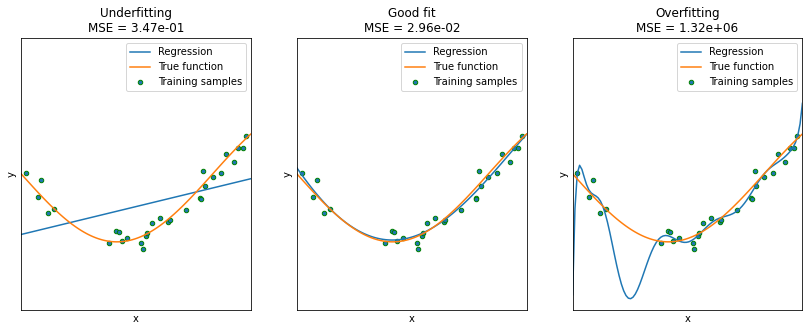
\includegraphics[width=0.9\textwidth]{figures/regression/overfitting.png} 
    \caption{Regression on a function with training examples. 
            The underfitting model is not complex enough to fit to the data well. 
            The overfitting model is too complex for the data.
            While the training error is lower for the overfitting model, 
            the overall performance of the overfitting model on previously unseen data 
            is worse than for the model with a good fit.
        }
    \label{fig:overfitting}
\end{figure}
  
To prevent overfitting while still getting good regression results, multiple network architectures need to be considered.
The networks proposed here were found by trail and error first, and later improved by hyperparameter analysis.

%TODO: Introduce NNs, normalzation, regularization, overfitting, underfitting.
% TODO: Regularization
% TODO: Normaliztation blabla

\section{Regression on fourier descriptor features}
\label{sec:Evaluation:fourier}

In the first approach, the features generated by the fourier descriptor were used to training.
Notable hyperparameters to the feature extractor here are the number of layers $l$ and the order of the fourier descriptor $o$.

The start and end height of the layers are chosen so that all the molecules in the dataset fully fit within $z_{min}$ and $z_{max}$.

The output shape of the descriptor will be an array of size $l \times (o * 4 - 1)$.
Generally, the bigger the number of fourier coefficients, the better the contour can be approximated.
However, an order that is chosen too high may increase the risk of overfitting, 
This problem is commonly referred to as "the curse of dimensionality".

A simple numerical approach to finding the order with the highest prediction accuracy is not necessarily viable in this case.
Since the ultimate goal is not to get the most accurate prediction possible, but instead discover which parts of 3d space 
are responsible for prediction, an order that offerers reasonable high accuracy without being subject too to much noise when explaining the 
prediction needs to be found. %TODO: Other reasons why order 10?

After various tests with multiple orders, an order of $k_{max} = 10$ seemed to be a good compromise between accuracy of description and accuracy of prediction.

The same problem is faced when defining the number of slices.
Here the problem becomes more tricky, since the number of slices seems to play a huge part in the architecture of the ANN used.
While the minimal number of slices should also be defined manually to allow for a proper reconstruction, the exact number of slices should be subject of a hyperparamter analysis.

%TODO: Hyperparameter analysis

Since every slice is composed of same kind of fourier coefficients, the first idea was to use convolution layers the decrease the dimensionality of the input.
Filters might be able to recognize structures in each of the slices, and applied them across the different slices.

Convolution layers heavily depend on the assumption that the relative location of features in matters.
Filter sizes were therefor chosen to correspond to the dimensions over which similarities in the structures of the features are expected.
In the case of fourier coefficients, the filter therefor were only stretched along the layer dimension, and not along the dimension of the fourier descriptors.

Multiple tests were performed with various filter sizes and convolution layers.
The regression accuracy was falling short of expectations, and the general shape of the network did not seem to change the prediction accuracy significantly.

\begin{figure} [h]
    \centering
    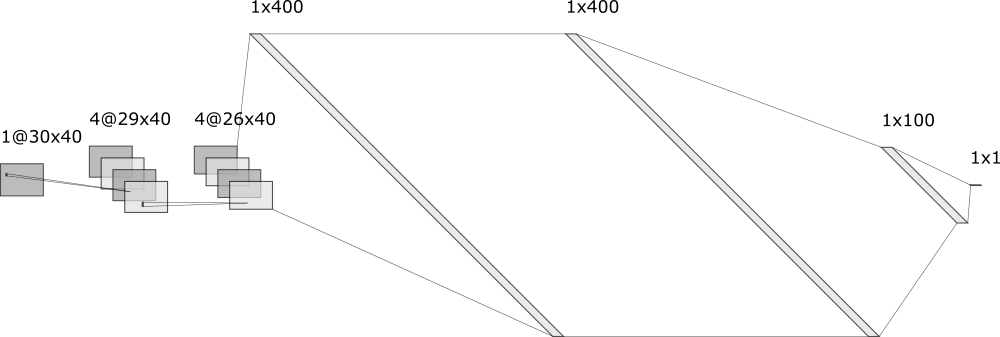
\includegraphics[width=0.7\textwidth]{figures/regression/fourier/cnn/fourier_conv_layout.png} 
    \caption{
        Architecture of the convolutional neural network used for predicting the activation barrier from fourier coefficients.
    }
    \label{fig:cnn-architecture}
\end{figure}

In first network architectures, overfitting was a mayor problem.
With regularization and other techniques the issue of overfitting could be reduced.
What became clear pretty early in the tests was that convolution layers did not improve prediction accuracy as expected.
When testing different filter configurations, the network performed best the smaller the filters got, and the fewer convolution layers were used.
In the end, the best performing Convolutional Neural Network found had two Convolution Steps with a filter size of $2 \times 1$ for the first layer, and a filter size
of $4 \times 1$ for the second layer \ref{fig:cnn-architecture}.
After the convolution layers 3 fully connected layers and the output layer followed.
Dropout and batch normalization layers were added in between to help with fighting overfitting.
The prediction accuracy of the CNN was similar yet slightly worse than the prediction accuracy achieved on autocorrelation features \cite{friederich_dos}.
The best CNN achieved a mean squared error over all test examples of $MAE=1.36$ and a coefficient of determination of $r^2=0.84$ \ref{fig:fourier_cnn}.
In comparison, the best neural network of \cite{friederich_dos} achieved a prediction accuracy of $MAE=1.12$ and $r^2=0.845$.

Since the space of possible network configurations is highly irregular, there is likely a network configuration using convolution layers 
that performs better than the one found here.
However all the tests performed were indicating that densely connected layers would achieve similar or higher accuracy.
The idea of convolution layers was therefore dropped early on, and instead the focus was shifted to optimizing a fully-connected architecture.

\begin{figure}[!htb]
    \minipage{0.1\textwidth}
    \endminipage\hfill
    \minipage{0.4\textwidth}
      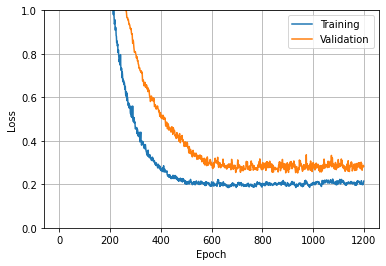
\includegraphics[width=1.0\textwidth]{figures/regression/fourier/cnn/lossCNN.png}
    \endminipage\hfill
    \minipage{0.4\textwidth}
      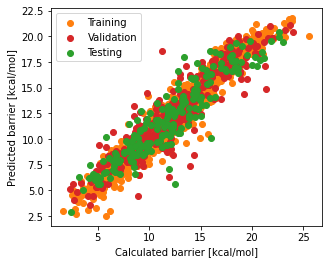
\includegraphics[width=1.0\textwidth]{figures/regression/fourier/cnn/scatterCNN.png}
    \endminipage\hfill
    \minipage{0.1\textwidth}
    \endminipage
    \caption{
        Loss while training the CNN. The jitter in the training loss during convergence is likely caused by the dropout layers. 
        The optimization goal was minimizing the mean squared error. 
        Training was performed on 80\% of the data.
        On the right are the predictions of the activation barrier in comparison to the real values ($MAE=1.36$, $r^2=0.84$).
    }
    \label{fig:fourier_cnn}
\end{figure}

Since previous research has proven that similar accuracy to the convolution approach can be achieved by learning from autocorrelation features,
the next idea was to use a transfer learning approach.
In a first step, the network would be taught to predict the autocorrelation features computed in \cite{friederich_dos}.
In a second step, the network is then extended to learn to predict that activation barrier \ref{fig:transferlearn}.
The hope was that teaching the network about autocorrelation features, the model would learn to recognize relevant properties of a catalyst.
In a second step, the entire network would then be trained to adapt specifically to the activation barrier.

\begin{figure} [h]
    \centering
    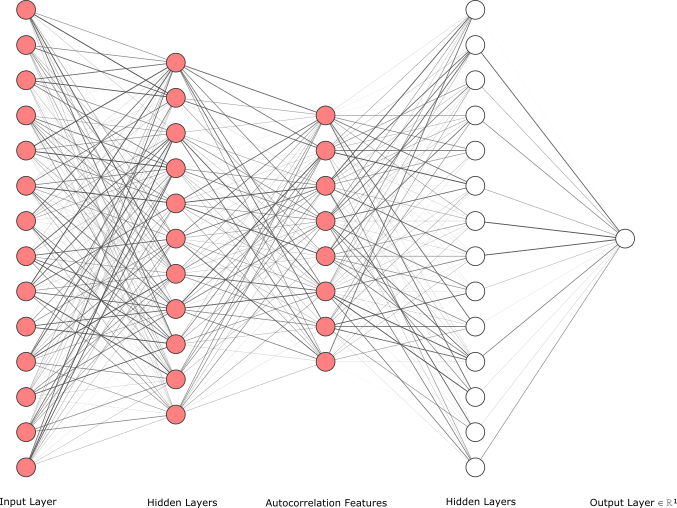
\includegraphics[width=0.7\textwidth]{figures/regression/fourier/nn.png} 
    \caption{Illustration of the transfer learning approach.
        In red the original model predicting autocorrelation features from the input is illustrated.
        In white the second part of the network, predicting the activation barrier from the autocorrelation features, is illustrated.
        Different sizes and amounts of hidden layers were tested. Here, single hidden layers are shown for illustration purposes.
    }
    \label{fig:transferlearn}
\end{figure}

Since the convolutional approach did not seem to improve results, a fully connected architecture predicting autocorrelation features from fourier coefficients 
was used.
Since there were 30 autocorrelation features used, the last layer of the network had a size of 30.
Findings about good hyperparameter, such as layer size, regularization and dropout rates, could be partly reused from the convolution step.
In the end, a network that predicted 30 independent autocorrelation features was found.
The network was able to predict some autocorrelation with very high accuracy. Specifically, the $T$ features and $I$ features were
predicted with an accuracy of $r^2 > 0.98$. 
Other features, such as $Z$ features, were lacking behind in accuracy, with the network only being able to reach accuracy of $r^2<0.96$ for some features.
The features the network was able to approximate well were also less important to the network found in \cite{friederich_dos}, while the features 
the network performed poorly on were the more important features \ref{fig:transfer_result}.

\begin{figure}[!htb]
    \minipage{0.32\textwidth}
      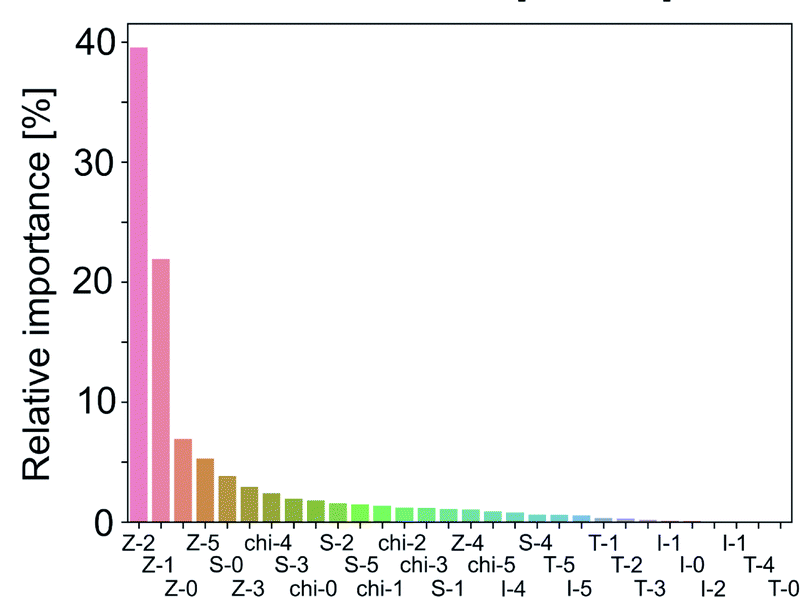
\includegraphics[width=1.0\textwidth]{figures/regression/fourier/importance_map.png}
    \endminipage\hfill
    \minipage{0.32\textwidth}
      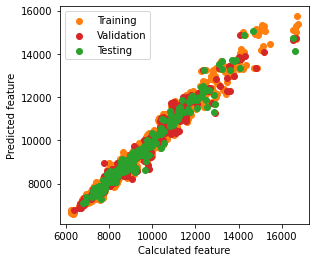
\includegraphics[width=1.0\textwidth]{figures/regression/fourier/transfer/scatterZ2.png}
    \endminipage
    \minipage{0.32\textwidth}
      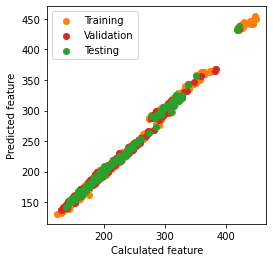
\includegraphics[width=1.0\textwidth]{figures/regression/fourier/transfer/scatterT0.png}
    \endminipage
    \caption{
    Left: Importance of features for the neural networks discussed in \cite{friederich_dos}.
    Middle: Prediction of Z-2 features from fourier features.
    Right: Prediction of T-0 features from fourier features. 
    The network was trained on 80\% of the data points.
    }
    \label{fig:transfer_result}
\end{figure}

After the network predicting the autocorrelation features was trained, the the transfer learning was started.
The last layers of model were removed, and replaced with newly initialized layers.
These newly added layers have and output size of 1 to allow for prediction of the activation barrier.
The best configuration found kept the first 3 layers of the original network, and then added 3 additional hidden layers and one output layer.
Regularization and normalization was used for some of the layers.
The model was then trained again with fourier coefficients as input and activation barriers as output.
Compared the convolution approach, the network took longer to converge, the overall regression accuracy improved.
The network achieved a $r^2=0.874$ and a $MAE=1.139$ when trained on 80\% of the data \ref{fig:transfer_final}.

\begin{figure}[!htb]
    \minipage{0.3333\textwidth}
      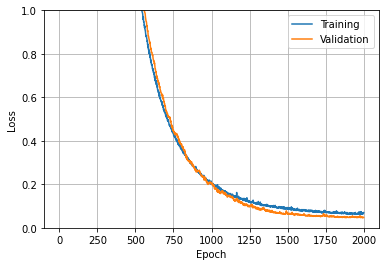
\includegraphics[width=1.0\textwidth]{figures/regression/fourier/transfer/lossTransferAutocor.png}
    \endminipage\hfill
    \minipage{0.3333\textwidth}
      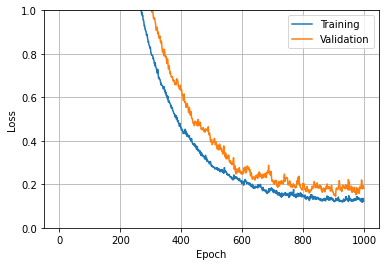
\includegraphics[width=1.0\textwidth]{figures/regression/fourier/transfer/lossTransferFull.png}
    \endminipage\hfill
    \minipage{0.3333\textwidth}
      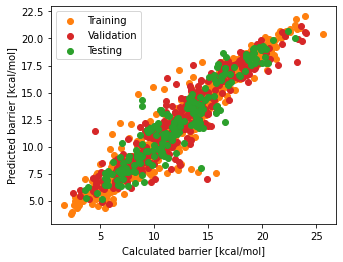
\includegraphics[width=1.0\textwidth]{figures/regression/fourier/transfer/scatterTransferFull.png}
    \endminipage
    \caption{
    Loss of the network being trained to predict autocorrelation features (right).
    The adapted network is then trained again to predict the activation barrier. The loss function in the middle shows the second training.
    The prediction accuracy has slight improved (right).  
    }
    \label{fig:transfer_final}
\end{figure}

In an attempt to find a better network architecture, a hyperparameter optimization was performed.
Hyperparameter optimization is a way of finding good hyperparameter for the underlying problem.
A searchspace need to be defined manually first, an optimization algorithm is then run to find good parameters within the search space.
Generally a bigger search space mean longer computation time for the hyperparameter algorithm.
The search space here was limited by the findings of manual hyperparamter tuning.
Notable optimization values given to the hyperparamter tuner were the number of convolution layers, 
the number and size of fully connected layers, the regularization rate of these layers, and the dropout rate for the layers.


\begin{figure}[!htb]
    \minipage{0.3333\textwidth}
      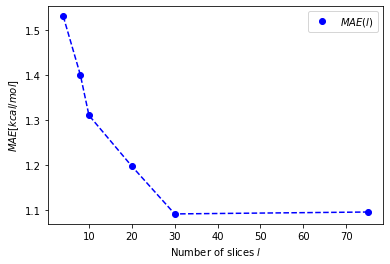
\includegraphics[width=1.0\textwidth]{figures/regression/fourier/mae_layer.png}
    \endminipage\hfill
    \minipage{0.3333\textwidth}
      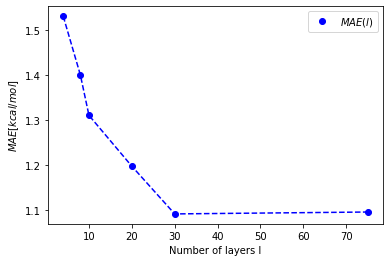
\includegraphics[width=1.0\textwidth]{figures/regression/fourier/r2_layer.png}
    \endminipage\hfill
    \minipage{0.3333\textwidth}
      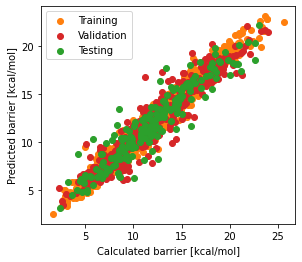
\includegraphics[width=1.0\textwidth]{figures/regression/fourier/scatterHyperparam.png}
    \endminipage
    \caption{
    The $r^2$ values and $MAE$ for different layer heights.
    For all layer heights a separate hyperparameter optimization wa run, resulting in different network architectures.
    All networks are trained using 80\% on the data. The $r^2$ scores and $MAE$ were evaluated later using a test dataset.
    The on the right the prediction of the best performing network found in the hyperparameter optimization step is plotted.
    The best network was found using a input layer height of $0.2 \AA$ resulting in $75$ layers. 
    The $MAE=1.096$ and $r^2=0.882$ are the highest accuracy so far.
    }
    \label{fig:fourier_final}
\end{figure}


In addition, multiple hyperparameter optimizations were performed for different layer heights $l$.
Since the layer heigh also changes the input size of the neural network, an assumption about the 
architecture across different layer heights is not feasible.
For ever layer height a separate hyperparamter optimization was run \ref{fig:fourier_final}.
The best hyperparameters found for every input site vary substantially.

After a certain layer height the prediction accuracy seems to no longer improve.
The step from 30 to 75 layers does not change the accuracy significancy, while more than doubling input size.
The small improvement in accuracy from 30 to 75 layers might not necessarily mean a higher overall classification accuracy of the network,
but could also be to randomness when selecting training and test examples or randomness during training.

The process shows that performing regression on fourier features is possible.
The accuracy however is not significantly higher than the accuracy achieved on graph convolutions.
Since the goal of this thesis is to learn from the 3D structure of the molecule, the similar performance 
indicates that the information learned from the 3d structure is limited.
This assumption is further validated by the fact that the transfer learning approach that 
basically eliminates spacial information about the network in the middle of the network, achieves similar accuracy to the 
network trained on features that do not include any information about the 3d structure.

Due to these results, a different feature extractor, SNAP, was developed.

\section{Regression on SNAP features}
\label{sec:Evaluation:snap}

Similar to the feature space for fourier coefficients, the size of the SNAP feature space is determined by two factors.
The first is the number of elements in the dataset.
The second is the resolution of the encoding for each type of element, defined by $n_{max}$ and $l_{max}$.

Other hyperparameters, such as the choice of radial basis functions, might influence the prediction accuracy further.

The number of radial basis functions $n_{max}$ and the maximum degree of spherical harmonics $l_{max}$ do both influence
the input dimension.
The ideal network architecture for different values will therefor vary too.
Since the values determine the accuracy with which accuracy the space is encoded, choosing these values purely 
based on which combination achieves the highest classification accuracy is not feasible.
The higher the degree of the spherical harmonics and radial basis functions, the more precise the element can be described.
The higher number of coefficients might however come at the price of noise when trying to explain the prediction later on.
A good balance between interpretability and accuracy was found with $l_{max}=n_{max}=3$. %TODO: Really? 

Hyperparameter analysis was performed on different combinations of $n_{max}$, $l_{max}$.
Since hyperparameter optimization is very computationally expensive, taking up to multiple days on modern high-performance 
server hardware, the number of combinations that could be explored is limited.

SNAP features are not fully rotationally invariant.
In order to allow the model to learn about the different possible rotations of the molecule, data augmentation was used.
In the hyperparameter optimizations performed here, 20 evenly spaced rotations of the molecule along the $z$-Axis were used.
The features for all of the 20 rotations was then fed into the model.
Tests with different augmentation steps showed that 20 augmentations seemed to be a good balance between 
accuracy and training speed.
Since the size of training examples rises linearly with the number of data augmentations,
high numbers of augmentations will drastically decrease training speeds.
This will in effect also reduce the speed of hyperparameter optimization.

\subsection{Normalization}

In a first step, the features generated by SNAP and the labels were normalized.
Normalize means scaling both labels and features independently so that mean is equal to $0$ and the standard deviation is equal to $1$.
Normalization is performed on each feature independently of each other.
This helps the network to generalize from the data better since no large biases have to be learned.

Since the data is normalized, the output from the network will not be the activation barrier directly.
Instead, the output needs to be scaled back to compute the performance of the network.

\subsection{Convolutional Neural Network}

Similar to the features generated by EFD, the output of SNAP can be shaped into a feature matrix again.
Here, each layer will correspond to one species of atoms.
Since the dataset the model is trained on consists of 12 different species of atoms, the feature matrix will have a height of 12.
Each row will then hold the coefficients describing the density of this species around the iridium center.
Depending on the choice of $n_{max}$ and $l_{max}$, the number of coefficients will change.

Since a coefficient of the $k$-th row will correspond to $c^k_{nlm}$, meaning every coefficient in the same colum has the same spacial meaning,
a convolutional neural network was the first idea to reduce the size of the input space and allow the network to learn structure in the input data.

Since not every molecule in the dataset consists of every atom, the input matrix will generally be sparse.
Rows that correspond to atoms not in the dataset will be filled with 0.
A filter that learns the general structure of the space and that is moved over the different species, therefor 
being able to ignore sparse inputs seemed to be a good choice.

Using a hyperparameter optimization to find the ideal filter size and number of convolution layers however showed
the a fully connected approach reaches higher accuracy than convolutional layers.
The hyperparameter optimizer not only gravitated towards a small amount of filters, but also towards 
the smallest possible filter size allowed in the hyperparameter space.

In further optimization the idea of convolution layers was therefor dropped in favour of fully connected layers.

\subsection{Fully connected neural network}

In a next step, hyperparameter optimization was focused on fully connected layers.
For different combinations of $n_{max}$ and $l_{max}$ hyperparameter optimizations were run.

The hyperparameter optimizer was allowed to choose between 1 to 6 hidden layers.
For each layer, the number of neurons, regularization rate and dropout rate could be chosen by the optimizer.
Additionally, the optimizer had the option to add a batch normalization layer after each of the layers.
The layers were then finished off with one neuron fully connected to the last hidden layer.

The activation function for each of the layer was fixed to Relu activations.

Hyperparameter analysis was then run using Keras Hyperband tuner.
Keras Hyperband is an  implementation of the Hyperband algorithm propsed in \cite{li2017hyperband}.
Hyperband focuses on an optimized search speed compared to other Hyperparameter optimization methods, such as
Bayesian Optimization. %TODO: Mehr?

Using the Hyperband Optimizer, the configurations discussed in the following sections were found.
Since the hyperparameter space was limited, for example to the use of relu activation functions,
the best performing models were then further enhanced manually.

\paragraph{Feature size}
The expectation was that the more accurate the density space would be described, the higher the prediction accuracy would be.
However after a full hyperparameter optimization on a variety of combinations of $n_{max}$ and $l_{max}$,
the differences in accuracy were not as significant as expected.
While increasing the number of $n_{max}$ coefficients seemed to increase the prediction accuracy,
overall the randoms of the training process seemed to have far higher influence on the models performance.
The infleunce of $n_{max}$ seemed to dominate over the influence of $l_{max}$.
Highest prediction accuracies where achieved by networks performing regression on features generated with $n_{max} > 6$.

Since hyperparameter searches for are very costly, taking up multiple days on modern day cloud-computing hardware,
hyperparameter analysis was run to an $l_{max} = 9$.
Significantly increasing $n_{max}$ might further improve prediction accuracy.

\begin{figure}[!htb]
  \minipage{0.3333\textwidth}
    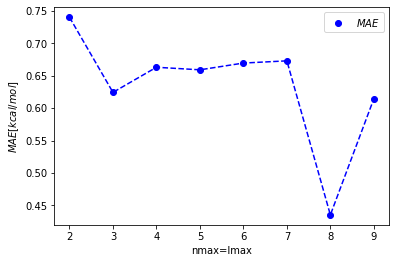
\includegraphics[width=1.0\textwidth]{figures/regression/snap/nmaxlmax.png}
  \endminipage\hfill
  \minipage{0.3333\textwidth}
    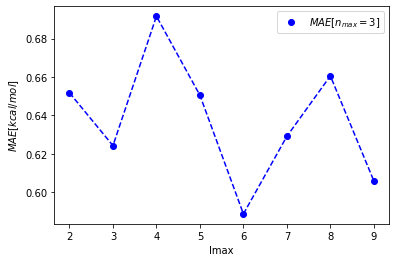
\includegraphics[width=1.0\textwidth]{figures/regression/snap/lmax.png}
  \endminipage\hfill
  \minipage{0.3333\textwidth}
    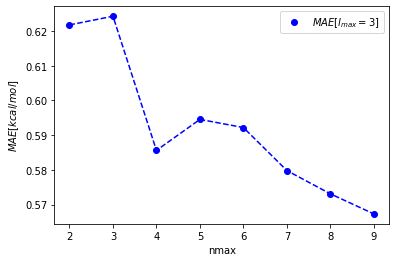
\includegraphics[width=1.0\textwidth]{figures/regression/snap/nmax.png}
  \endminipage
  \caption{
  The $r^2$ values and $MAE$ for different $n_{max}$ and $l_{max}$.
  The network architecture was optimized separately for each combination using hyperparameter optimization.
  The best network was found for $n_{max}=8$ and $l_{max}=8$ with a $MAE=0.435$ and a $r^2 = 0.978$.
  This could be an outlier due to a falling into a good local minima during either training or hyperparameter optimization.
  }
  \label{fig:snap_hyperparameter}
\end{figure}

\paragraph{Cutoff sphere}
All hyperparameter searches were run with with a cutoff radius $r_{cut} = 20 \AA$.
This cutoff sphere is large enough to fully fit every element of the dataset into it.
However, due to the nature of the radial basis functions used, the resolution of atoms 
further away from the center will decrease.
Tests with different cutoff radii were therefore performed.
The tests were run on the network architectures found by hyperparamter optimization.

For every configuration of $n_{max}$ and $l_{max}$, a networks were trained for a variety 
of tests splits and data augmentation steps.
These networks were then evaluated by their performance with respect to the cutoff radius.

Up to a cutoff radius of $10 \AA$, the mean network performance improved. %TODO: Rich
At a training fraction of 80\%, the mean classification error among 
all networks decreased from $0.889 \AA$ for a cutoff radius of $5 \AA$ to 
$0.801 \AA$ for a cutoff radius of $10 \AA$.
From there however, increasing the cutoff radius did not improve the accuracy further.
This lead to the hypothesis that atoms closer to the metal center are more important to the activation barrier than atoms further away from the center.
This hypothesis could also explain the slight increase in prediction error when further increasing the cutoff radius.
Since the resolution of the feature space is limited, increasing the cutoff radius might have decreased the accuracy 
with which the inner atoms are described in the features, thus decreasing the prediction accuracy.

To verify this hypothesis, a second experiment was run.
Here, all atoms outside a cutoff sphere were removed from the element before passing it on to the encoder.
The atoms were then encoded with a cutoff radius $2 \AA$ higher than the cutoff sphere to allow for a proper 
encoding of atoms just inside the cutoff sphere.
The networks were once again trained with the hyperparameters found in the initial hyperparameter analysis.
The training was run for cutoff spheres of $2\AA, 4\AA, 6\AA, 10\AA, 15\AA, 20\AA$ resulting in $r_{cut}$ 
of $4\AA, 6\AA, 8\AA, 12\AA, 17\AA, 22\AA$.
For $r_{cut}=4$, no prediction was possible and the networks just predictied the mean of the data.
This was to be expected since at this cutoff radius, only 20\% of the elements are encoded into the features.
However for $r_{cut}=8$ the mean MAE over all networks trained on 80\% of the data was at $MAE = 0.834 \AA$. 
A $r_{cut} = 8$,resulting in a cutoff sphere of $6 \AA$, 96\% of the atoms are included in the data. 
The remaining 4\% fall outside of the cutoff sphere and are therefore ignored. 

For $r_{cut}=12$ the mean MAE over all networks trained on 80\% of the data was at $MAE = 0.836 \AA$. 
A this cutoff radius, 100\% of the atoms are included in the data.
While this accuracy is marginally higher, the difference is so small that is could 
simply be explained by the optimizer falling into different local minima compared to $r_{cut}=8$. 

This lead to the conclusion that, while all atoms in the dataset seem to have an effect on the prediction,
choosing a tight $r_{cut}$ achieves the best prediction accuracies.
When looking at the nature of the encoding, this intuition is verified.
Empty space that is indirectly included into the enocoders features.
Since the encoder will try to encode a density of 0 in these regions, the features 
need to include this information, and competing with the relevant information about the element.
From now on, all cutoff radii will therefor be chosen at $r_{cut} = 12 \AA$.

\begin{figure}[!htb]
  \minipage{0.3333\textwidth}
    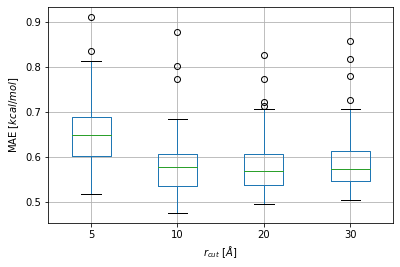
\includegraphics[width=1.0\textwidth]{figures/regression/snap/cut-all.png} %TODO: REPLACE!!!!
  \endminipage\hfill
  \minipage{0.3333\textwidth}
    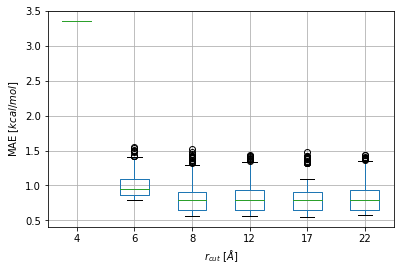
\includegraphics[width=1.0\textwidth]{figures/regression/snap/cut-sphere.png}
  \endminipage\hfill
  \minipage{0.3333\textwidth}
    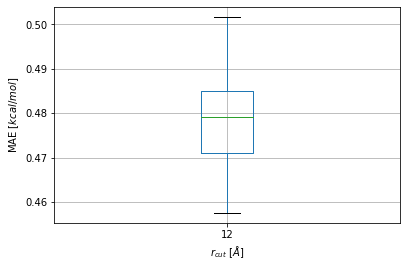
\includegraphics[width=1.0\textwidth]{figures/regression/snap/cut_12.png} %TODO: REPLACE!!!
  \endminipage
  \caption{
  Networks trained on different cutoff radii. All networks are trained on a train fraction of 80\%.
  The figures on the left and right show networks being trained on all atoms in the dataset.
  For the figure in the middle, networks were trained on all data within a sphere the size of
  $r_{cut} - 2$. Atoms outside this sphere where not encoded in the density space.
  }
  \label{fig:snap_hyperparameter}
\end{figure}


\paragraph{Sensitivity to rotation}
Since snap features are not fully rotationally invariant, the networks ability to abstract rotation from the input is crucial.
In order to teach the network about the possible rotations of an element, 
the element is augmented by rotating it around the remaining axis of freedom, the $z$ axis.
For every augmentation step, the rotated element is added to the training data.
Tests with different augmentation steps were performed.
All networks were trained on the previously found hyperparameters.
The augmentation steps ranged from 5 evenly spaced rotations to 100 evenly spaced rotations.
Both the training and the test data was augmented to allow for learning from the augmented data
as well as to validate if the network was actually able to abstract away rotations.

Even with only 5 data augmentation steps the networks achieved a mean prediction error of $MAE = 40 \AA$.
The mean error over all networks decreased up to 40 augmentation steps.
After 40 augmentation steps no further decrease in mean prediction error was observed ~\ref{fig:snap_roation_out}.
For networks with higher data augmentation steps, the stability of the networks when trained on small train splits was higher.

The stability higher stability of networks with larger data augmentations is an interesting property.
While the hope was that higher numbers of data augmentation would allow the network to better abstract away rotation from the
element, the results do not seem to support that hypothesis.
Comparing the prediction of the network for different elements, the differences in prediction however is
very similar between networks trained on 5 data augmentations and networks trained on 60 data augmentations.
One interpretation here would be that the additional data points generated by augmenting the data help training the network,
rather than teaching it about the different possible rotations of the network.
This might explain why especially for lower train fractions the prediction accuracy is improved by more data augmentations.

One way to verify this theory is to use transfer learning to pretrain the network.
Since only the calculation of the activation barrier is costly, but not the generation of more elements,
in the future the network might be pretrained on properties that are easy to compute with a large dataset of catalysts.
This idea is further explored in \ref{ch:outlook}.

\begin{figure}[!htb]
  \minipage{0.3333\textwidth}
    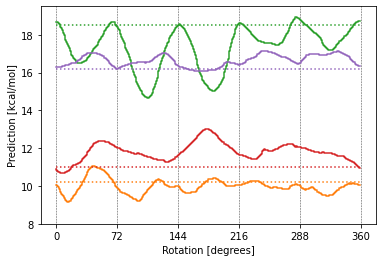
\includegraphics[width=1.0\textwidth]{figures/regression/snap/aug-5steps-30per.png}
  \endminipage\hfill
  \minipage{0.3333\textwidth}
  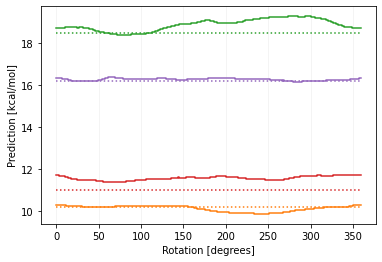
\includegraphics[width=1.0\textwidth]{figures/regression/snap/aug-30steps-30per.png}
  \endminipage\hfill  
  \minipage{0.3333\textwidth}
    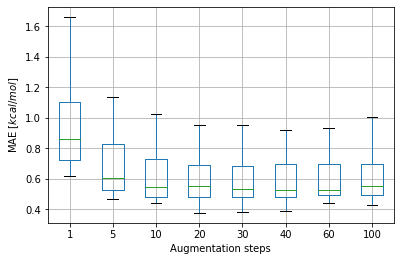
\includegraphics[width=1.0\textwidth]{figures/regression/snap/augmentation.png}
  \endminipage\hfill
  \caption{
  The predictions for a network on SNAP features for $n_{max}=9, l_{max}=3$ trained with 5 data augmentation steps (left) 
  and 20 augmentation steps (middle) for 4 randomly selected samples. 
  The continuos line is the prediction of the network, the dotted line is the calculated barrier.
  The networks were trained on a train split of 70\%.
  On the right are the results for multiple models trained on different augmentation steps.
  All networks are trained on the same network architecture, at different train fractions.
  }
  \label{fig:snap_roation}

\end{figure}


\paragraph{Results}

Even with slight variations in prediction accuracy, the overall results of regression performed on SNAP features is still promising.
All models found during hyperparameter optimization for different $n_{max}, l_{max}$ were able to predict the reaction barrier with higher accuracy than any model so far.
With the best models for $l_{max}=n_{max}=8$ achieving accuracies of $MAE=0.435 kcal/mol$ and $r^2=0.978$.
The hyperparameter optimization was performed on a training split of 80\%.

By manually improving the model after hyperparameter optimization, the accuracy could be increased further.
This indicates that a bigger hyperparamter space or a smaller step size of the optimizer towards the local minima can 
improve the results further.

The best network found after manual adjustment of the hyperparameters was at $n_{max}=l_{max}=3$.
It achieved an accuracy of $MAE=0.376 kcal/mol$ and $r^2=0.980$ on a train split of 80\%.
The network used a total of 3 hidden fully connected layers, with an increasing number of neurons.
BatchNormalization and dropout layers were used between the fully connected layers.
Their placement was determined by the hyperparameter optimizer.
Since the hyperparameter optimizer was only allowed to choose a between a limited number 
of regularization rates and dropout rates, and also a limited number of batch size for training,
optimization of these values manually further increased accuracy.

Compared to other modes of encoding the data, SNAP seems to be especially susceptible to outliers.
For all models, the regression accuracy is heavily influenced by a small number of samples with poor precision.
Since the split between training and test dat is random, the overall accuracy of the model is 
heavily influenced by the selection of samples in the test data.
Improving the networks stability to outliers could further increase regression accuracy.


\section{Comparison}
\label{sec:Evaluation:Comparison}

The neural networks proposed here were able to predict the activation barriers with high accuracies.
In \cite{friederich_dos}, different Machine Learning approaches to the regression problem were introduced.
While the dataset was the same, the features extracted from the molecules were different.
The comparison of the results from \citetitle*{friederich_dos} and this thesis is therefor more 
a comparison of feature extractors, and not a comparison of machine learning methods or network architectures.

Their best neural network trained on 80\% of the data achieved a prediction accuracy of $MAE = 1.12 kcal/mol$ and a 
coefficient of determination of $r^2 = 0.845$.
The neural network was 4 layers deep and trained on their autocorrelation features.
Autocorrelation features extract features from a graph representation of the chemical structure, but neglect the 
3d structure of the molecule \cite{friederich_dos}.
The best prediction accuracy was however in a yet unreleased paper by  a graph convolution neural network (GNN) on 
a graph structure of the molecule.
It achieved an accuracy of $MAE = 0.571 kcal/mol$ and $r^2=0.964$.
These are the highest accuracies achieved on this dataset yet.
While this was the state-of-the-art  to compare the models in this thesis to, the main objective was not to beat these numbers.
The goal was rather to achieve similar performance with a feature descriptor that allowed for a mapping back from feature space to 3d space.
This allows for an extensive interpretation of the results, which is impossible with current features.
The SNAP features however not only allow for this analysis, but are also able to beat the accuracy of GNN models.
Another important metric is the performance of the networks for different sizes of training data.
The models performance will therefore be compared by their accuracy for different test split sizes.
\\
The first approach regression was using LEFD features.
When training on 80\% of LEFD features, the best neural network achieved an accuracy of $MAE = 1.096 kcal/mol$ and $r^2=0.882$.
While the accuracy is slightly higher than the best neural network in \cite{friederich_dos}, it still falls short 
of the GNN.
Interestingly, the accuracy of the model is very similar to the accuracy achieved by the neural network trained on autocorrelation 
features.
Additionally the autocorrelation features could be approximated from the LEFD features reasonably well.
This could indicate that LEFD features and autocorrelation features describe
similar information about the element that is relevant to the activation barrier.
\\
The best models trained on SNAP features were able to achieve accuracies well below the $0.5 kcal/mol$ barrier.
While the final accuracies are heavily dominated by outliers, models trained on SNAP features were consistently
able to achieve accuracies better than the best model so far.
